\documentclass[14pt,margin=0.5in,innermargin=0in,blockverticalspace=-0.1in,colspace=-1.0cm]{tikzposter}
\geometry{paperwidth=841mm,paperheight=594mm}
\usepackage[utf8]{inputenc}
\usepackage{lmodern}
\usepackage{anyfontsize}
\usepackage{csquotes}
\usepackage{amsmath}
\usepackage{amsfonts}
\usepackage{amsthm}
\usepackage{amssymb}
\usepackage{mathrsfs}
\usepackage{graphicx}
\usepackage{adjustbox}
\usepackage{enumitem}
\usepackage{xcolor}
\usepackage[backend=biber,style=numeric,sorting=none]{biblatex}
\usepackage{durham-theme}
\usepackage{mwe} % for placeholder images
\usepackage{tcolorbox}
\usepackage{multicol}

\usepackage{caption}
\captionsetup[figure]{font=normal,labelfont=bf}

\addbibresource{references.bib}

% set theme parameters
\tikzposterlatexaffectionproofoff
\usetheme{DurhamTheme}
\usecolorstyle{DurhamStyle}

\usepackage[scaled]{helvet}
\renewcommand\familydefault{\sfdefault} 
\renewcommand{\vec}[1]{\bm{#1}}
\newcommand{\Tr}{\text{Tr}}
\usepackage[T1]{fontenc}

\title{Megapixel Image Generation with Step-unrolled Denoisng Autoencoders}
\author{\textbf{Alex F. McKinney}\textsuperscript{1},
\textbf{Chris G. Willcocks}\textsuperscript{1,2} 
}
\institute{\textsuperscript{1}Department of Computer Science, Durham University\\
            \textsuperscript{2}Project Supervisor
            }
\titlegraphic{
\includegraphics[width=0.16\linewidth]{durham-logo.png}}

% begin document
\begin{document}
\maketitle

\centering
\block{}
{
    \vspace{-2.5cm}
    \centering
    \begin{tikzfigure}
        \includegraphics[width=1.0\linewidth]{samples.png}
    \end{tikzfigure}
    \captionof{figure}{
            \centering
            $1024 \times 1024$ samples from our FFHQ1024 model. Resulting
            samples are diverse and of high-fidelity. Each sample was generated
            in $\approx 2$ seconds on a consumer-grade GPU (GTX 1080Ti), in
            contrast to existing approaches at this resolution, which take
            minutes to generate. To our knowledge, this is the fastest
            generating, non-adversarial framework at this resolution.
        }
    \vspace{0.5cm}
    \begin{scope}[line width=\titlelinewidth,]
    \draw[color=colorOne!30!colorOne,round cap-round cap]
    (\titleposleft,0)--(100,0);
    \end{scope}
}

\begin{columns}

    \column{0.3}
    \block{}{
        \vspace{-1cm}
        \begin{tcolorbox}[boxsep=0pt,top=0cm,adjusted title={\Large
            Background},colbacktitle=colorOne]
        \begin{tikzfigure}
            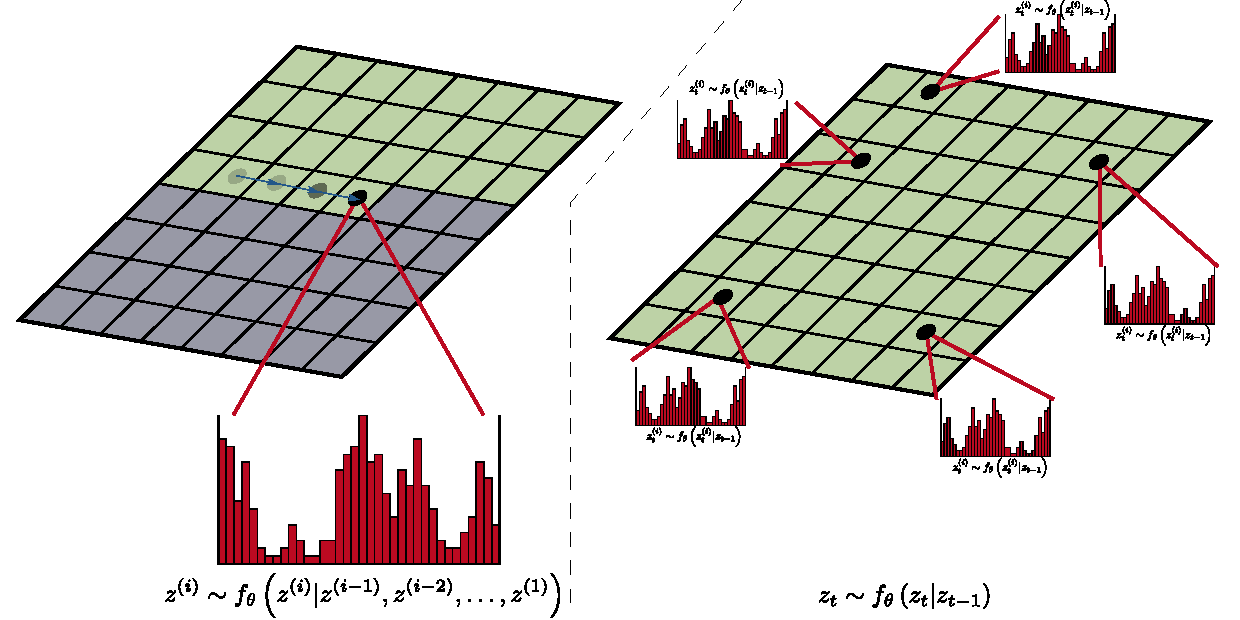
\includegraphics[width=1.0\linewidth]{AR-NAR.pdf}
        \end{tikzfigure}
        \vspace{-0.5cm}
        \captionof{figure}{
                Autoregressive sampling (left) is defined in terms of the
                probabilistic chain rule, meaning that sampling is done
                iteratively -- one element at a time -- so not to violate
                causality. Non-autoregressive sampling (right) does not have
                such constraints, and can sample an arbitrary number of elements
                in parallel. Crucially, this means the iteration complexity of
                sampling does not scale directly with data dimensionality, allowing
                massive scaleability. In addition, it can use the full context
                available to it, in order to make predictions, allowing for
                better quality samples and more flexible inpainting. Despite
                such advantages, non-adversarial, non-autoregressive generative
                models have not seen widespread adoption, due to requiring
                many sampling steps -- potentially thousands.
            }
        
        \begin{tikzfigure}
            \includegraphics[width=0.99\linewidth]{recon.pdf}
        \end{tikzfigure}
        \vspace{-1.0cm}
        \captionof{figure}{
                VQGAN is used to reduce computational requirements for training
                and sampling of our generator model SUNDAE. It acts as a
                compression model, reducing the spatial resolution at which we
                operate over. However, VQGAN does not always faithfully
                reproduce the input image, though outputs are perceptually
                valid. For example, left shows a change in eye colour and the
                concealment of a piercing by adjusting hair position. Middle has
                its hair texture changed. Right has piercings removed and text
                corruption. Despite this, VQGAN is the only model capable of
                producing the compression rates we need.
            }
            
        \end{tcolorbox}
    }
    
    \column{0.4}
    \block{}{
        \vspace{-1cm}
        \begin{tcolorbox}[boxsep=0pt,top=0cm,adjusted title={\Large Proposed Method},colbacktitle=colorOne]
        \begin{tikzfigure}
            \includegraphics[width=0.99\linewidth]{overall.pdf}
        \end{tikzfigure}
        \vspace{-0.5cm}
        \captionof{figure}{
                An overview of the SUNDAE training and sampling of discrete
                latent representations. Above the dashed line represents the
                process for training, whereas below the dotted line represents
                the sampling process. The training process begins by sampling
                $\mathbf{z} \sim \mathcal{L}$ and then sampling from the
                corruption distribution $q(\mathbf{z}_0 \vert \mathbf{z})$.
                SUNDAE then denoises for 2 to 3 steps, computing the
                cross-entropy loss at each step in the chain which is
                subsequently averaged to produce a final loss. Sampling begins
                by obtaining $\mathbf{z}_0$ from a uniform prior and iteratively
                denoising for more steps than trained with. At each step in the
                chain, the sample $\mathbf{z}_t$ can be decoded by the VQGAN
                decoder $G$ to obtain $\mathbf{y}_t$. We found SUNDAE to easily
                outspeed prior (non-adversarial) autoregressive and
                non-autoregressive models, using typically 50-100 steps during
                sampling, or in about 2 seconds.
            }
        %\vspace{1cm}

        \begin{minipage}{0.49\linewidth}
        \begin{equation}
            x
        \end{equation}
        \end{minipage}
        \begin{minipage}{0.49\linewidth}
        \begin{equation}
            x
        \end{equation}
        \end{minipage}
        \vspace{1cm}
        
        The objective of this project was to push the efficiency of generative
        models to their limit and expand the array of non-autoregressive methods
        for image generation. By combining various methods -- each at the
        pinnacle of efficiency in their respective areas. These include VQGAN, a
        vector quantization model with an unparalleled rate of compression;
        hourglass transformers, a highly scaleable attention model; and SUNDAE,
        a fast, non-autoregressive text generative model.

        Our primary contributions are as follows:
        \begin{itemize}
            \item
                The development of a non-autoregressive, non-adversarial
                generative modelling framework with extremely flexible sampling
                including self-correction and arbitrary inpainting pattern
                capabilities. The model can be directly configured for both low-
                and high-step sampling scenarios, resulting in high quality and
                diverse samples in mere seconds of sampling time.

            \item
                Modifications to SUNDAE and hourglass transformers to be more
                suited for the modelling of multi-dimensional discrete data. Though
                applied to discrete latents in our work, the modifications are
                also applicable in a wider context, such as to pixel-level
                modelling. We also demonstrate the superiority of hierarchical
                transformers -- forming a key component in the scalability of
                our approach. 
            \item
                The scaling of VQGAN to extremely high resolution images of
                human faces. $1024 \times 1024$ images far exceeds resolutions
                achieved in prior work. This ultimately allowed for the
                \textbf{generation of megapixel images in as few as two seconds}
                on a consumer-grade GPU when combined with our fast and scalable
                generative framework. This is in contrast to prior
                autoregressive methods and non-autoregressive diffusion methods
                that take minutes to generate, or have not scaled to such
                resolutions entirely.

        \end{itemize}
        \end{tcolorbox}
    }

    \column{0.3}
    \block{}{
        \vspace{-1cm}
        \begin{tcolorbox}[boxsep=0pt,top=0cm,adjusted title={\Large Results},colbacktitle=colorOne]
        \begin{tikzfigure}
            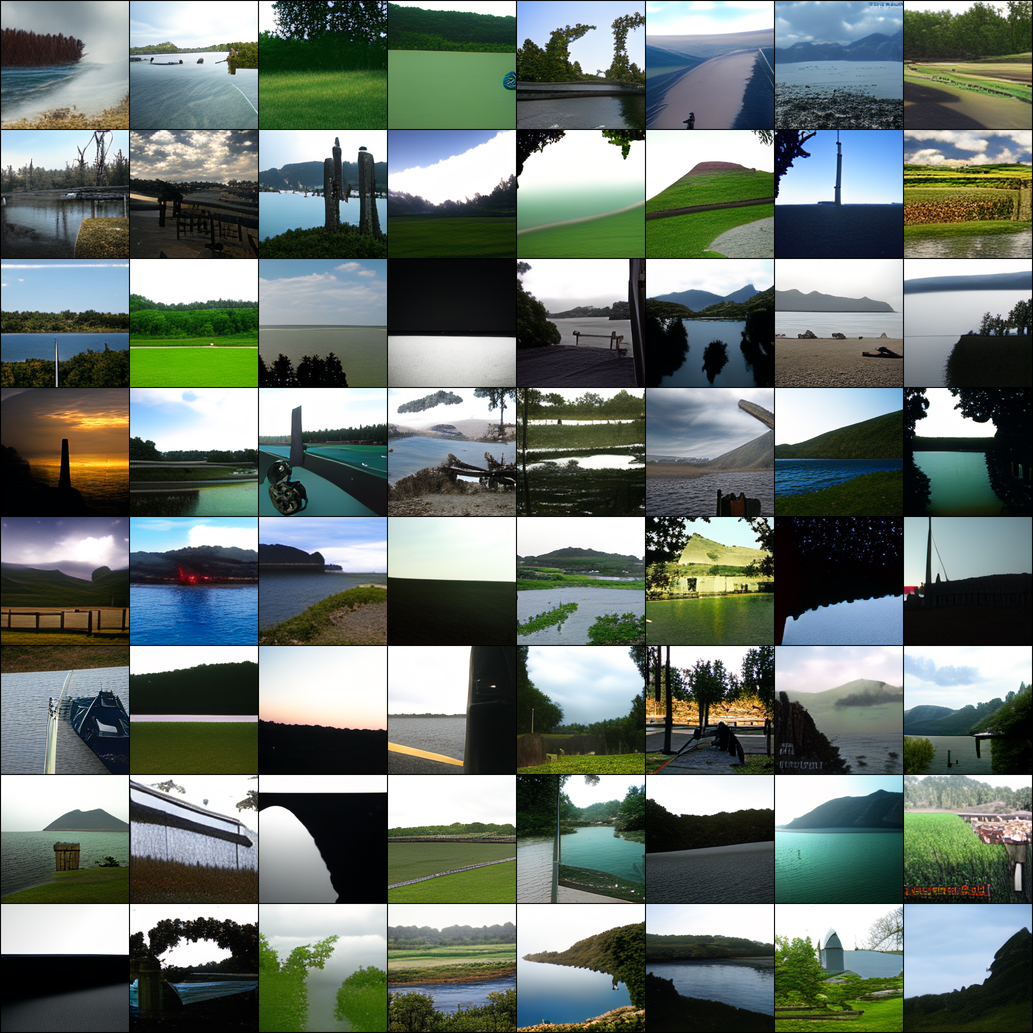
\includegraphics[width=0.49\linewidth]{imagenet-lakeside.png}
            \hfill
            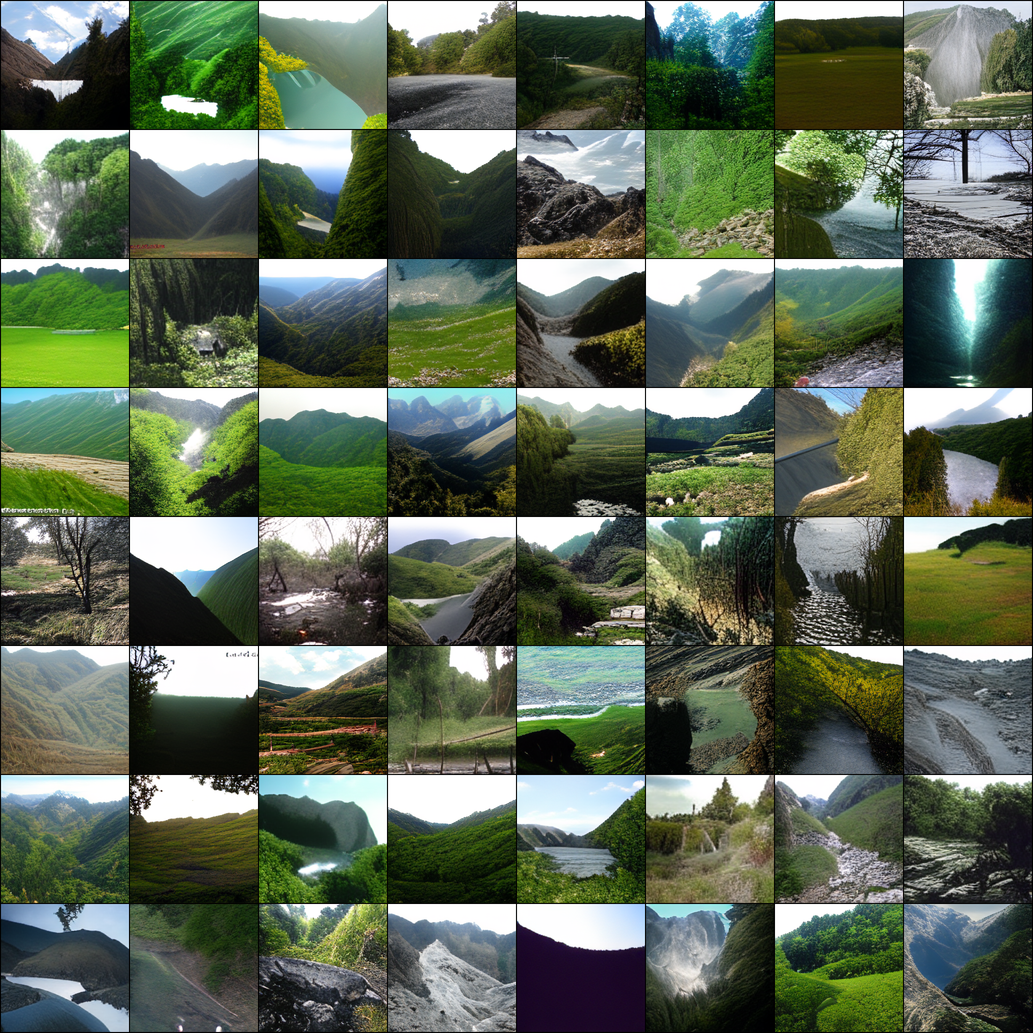
\includegraphics[width=0.49\linewidth]{imagenet-valley.png}
            \captionof{figure}{
                $256 \times 256$ class-conditioned samples on
                ImageNet. The left batch of samples are from the class
                ``Lakeside'' whereas the right batch are from the class
                ''Valley''. We trained on the full 1000 classes available in the
                dataset, using a simple embedding vectors as a conditioning
                signal. We note, that our approach can easily be extended to
                obtain a powerful text-to-image generator, by using text prompts
                as a conditioning signal.
            }
        \end{tikzfigure}
        
        \vfill

        \begin{tikzfigure}
            \includegraphics[width=0.49\linewidth]{inpaint-rand.png}
            \hfill
            \includegraphics[width=0.49\linewidth]{inpaint-block.png}
            \captionof{figure}{
                Representative inpainting results on FFHQ1024 using our trained
                model. We demonstrate the superiority of non-autoregressive
                methods for inpainting by using arbitrary inpainting masks,
                including completely random (Left) and large block masks
                (Right). Such patterns are difficult to inpaint with
                autoregressive models, and cannot utilise the full context
                available to them.
            }
        \end{tikzfigure}
        \end{tcolorbox}
    }

    % TODO: potentially a manual bibliography of relevant literature
    \block{}{
        \vspace{-1cm}
        \begin{tcolorbox}[boxsep=0pt,top=0cm,adjusted title={\Large
            References},colbacktitle=colorOne]
        \nocite{*}
        \vspace{0.4cm}
        \begin{footnotesize}
        \printbibliography[heading=none]
        \end{footnotesize}
        \end{tcolorbox}
    }
\end{columns}
\end{document}
